\documentclass[a4paper,12pt, master]{etf}

\usepackage[intlimits]{amsmath}
\usepackage{amsmath, amsfonts, amssymb, graphicx}

\usepackage[serbian]{babel}
\usepackage[T1]{fontenc}
\usepackage[utf8]{inputenc}
\usepackage{graphicx}

\addto\captionsserbian{\renewcommand{\bibname}{Literatura}}

\title{Implementacija}
\author{Lazar Caković}
\indeks{3083/2016}
\date{septembar 2018.}
\mentor{Prof. dr Lazar Saranovac}
\predmet{}

\begin{document}

	\maketitle

	\tableofcontents

	\listoffigures

	\newpage

	\chapter{Apstrakt}

	\newpage

	\chapter{Uvod}

	\newpage

	\chapter{Protokol}

	\section{OSI model}

	Open Systems Interconnection model (OSI model) je konceptualni model koji karakterise i
	standardizuje komunikacione funkcije u telekomunikacionim ili kompjuterskim sistemima, i to bez
	obzira na unutrasnju strukturu uredjaja ili njihovu tehnologiju. Cilj ovog modela je da se
	postigne kompatibilnost razlicitih komunikacionih sistema sa standardnim protokolima
	komunikacije. OSI model razdvaja komunikacione sisteme u apstraktne slojeve. Originalna verzija
	modela ima sedam slojeva.

	Sloj unutar modela sluzi sloj iznad njega, i koristi sloj ispod njega u hijerarhiji. Na primer,
	sloj koji postize komunikaciju preko mreze bez gresaka, sluzi aplikacijama iznad koje ga
	koriste, i to dok poziva jednostavne funkcije za prijem i predaju paketa na mrezi. Dve instance
	istog sloja su vizualizovane tako sto su povezane horizontalno u istom sloju.

	Ovaj model je proizvod Open Systems Interconnection projekta u International Organization for
	Standardization (ISO), i ima oznaku ISO/IEC 7498-1.

	\#\# [lazarc] slika svih slojeva u osi modelu

	Na svakom nivou N, dva entiteta na komunikcionim uredjajima razmenjuju jedinice protokola (PDU
	- protocol data units) pomocu sloja N protokola. Svaki PDU sadrzi podatke od interesa (payload)
	(SDU - service data unit), zajedno sa zaglavljima koji odgovaraju protokolu.

	Obrada podataka izmedju dva uredjaja koji su OSI-kompatibilni se odvija u sledecim koracima:
	\begin{itemize}
		\item Podaci koji se prenose se formiraju na najvisem sloju u uredjaju koji predaje podatke
		na mrezi (sloj N) u jedinicu protokola (PDU).
		\item PDU se prosledjuje sloju N-1, gde je poznat kao SDU.
		\item Na sloju N-1 se na SDU dodaju zaglavlja, na osnovu cega se formira PDU za sloj N-1.
		Nakon cega se prosledjuje na sloj N-2.
		\item Ovaj postupak se ponavlja sve dok se ne dostigne najnizi sloj u modelu, nakon cega se
		podaci prenose ka uredjaju koji prima podatke.
		\item Na strani prijemnog uredjaja se podaci prenose od najnizeg sloja u modelu, do
		najviseg, gde se serije SDU struktura uspesno obradjuju, pri cemu se skidaju zaglavlja sa
		svakog sloja, dok se ne dostigne najvisi sloj u modelu, nakon cega su dostupni sirovi
		podaci.
	\end{itemize}

	\#\# [lazarc] dodati jos nesto o ovome ukoliko se nadje.

	\subsection{Sloj 1: Fizicki sloj (Physical Layer)}

	Fizicki sloj je odgovoran za prenos i prijem nestrukturiranih sirovih podataka izmedju uredjaja
	i fizickog medijuma za prenos. On pretvara digitalne bitove u elektricne, radio ili opticke
	signale. Specifikacije sloja definisu karakteristike poput nivoa napona, fizicke brzine prenosa
	podataka, maksimalne udaljenosti prenosa i fizickih konektora. Ovo ukljucuje raspored pinova,
	napona, linijske impedanse, specifikacije kablova, vremenskih signala i frekvencije za bezicne
	uredjaje. Kontrola brzine bitova se vrsi na fizickom nivou i moze definisati nacin komunikacije
	kao simpleks, polu dupleks ili dupleks komunikaciju. Komponente fizickog sloja mogu se opisati
	u smislu topologije mreze. Bluetooth, Ethernet i USB, sve imaju specifikacije za fizicki sloj.

	\subsection{Sloj 2: Sloj veze (Data Link Layer)}

	Sloj veze podataka obezbedjuje prenos podataka izmedju dva cvora u komunikaciji - vezu izmedju
	dva direktno povezana uredjaja na mrezi. Ovaj sloj otkriva i eventualno ispravlja greske koje
	se mogu javiti u fizickom sloju. On definise protokol za uspostavljanje i prekid veze izmedju
	dva fizicki povezana uredjaja. Takodje, definise protokol za kontrolu protoka izmedju njih.

	IEEE 802 standard deli sloj veze na dva podsloja:
	\begin{itemize}
		\item \textbf{Kontrola pristupa medijumu (MAC - Medium access control):}
		\#\# [lazarc] [prevod]
		odgovorna je za kontrolu nacina na koji uredjaji na mrezi dobijaju pristup medijumu i
		dozvolu za prenos podataka.
		\item \textbf{Kontrola logicke veze (LLC - Logical link control):}
		\#\# [lazarc] [prevod]
		odgovorna je za identifikaciju i enkapsulaciju slojeva mreznog protokola, i kontrolu
		gresaka i sinhronizaciju paketa koji se salju.
	\end{itemize}

	MAC i LLC slojevi IEEE 802 mreznog standarda kao sto su 802.3 Ethernet, ili 802.11 Wi-Fi su
	slojevi veze (data link layer).

	Point-to-Point Protocol (PPP) - je protokol sloja veze koji radi na nekoliko razlicitih
	fizickih slojeva, kao sto su sinhrone ili asinhrone serijske linije.

	\subsection{Sloj 3: Mrezni sloj (Network Layer)}

	Mrezni sloj obezbedjuje funkcionalno i proceduralno sredstvo prenosa sekvenci podataka
	promenljive duzine, koji se nazivaju jos i paketi, od jednog cvora do drugog, poveznih u
	"razlicite mreze". \#\# [lazarc] [prevod] \#\# Mreza je medijum na koji moze biti povezano vise
	cvorova, u kom svaki cvor ima adresu i koji dozvoljava cvorovima povezanim sa njim da prenose
	poruke ka ostalim cvorovima, i to samo dajuci sadrzaj poruke i adresu cvora na koji poruka
	treba da bude dostavljena, omogucavajuci mrezi da nadje nacin da isporuci poruku odredisnom
	cvoru, eventualno ga usmeravajuci kroz sredisnje cvorove (uredjaje koji su izmedju dva uredjaja
	koji pokusavaju da komuniciraju). Ako je poruka prevelika da bi se prenela sa jednog uredjaja
	na drugi samo koriscenjem sloja veze (Data Link Layer), mreza moze preneti podatke tako sto ce
	ih podeliti u nekoliko delova na jednom uredjaju, poslati delove nezavisno, i onda spojiti
	delove na drugom uredjaju. Pri cemu moze, iako nije uvek potrebno, prijaviti greske u isporuci.

	Isporuka poruka na mreznom sloju nije garantovano pouzdana. Mrezni sloj moze pruziti pouzdanu
	isporuku poruka, ali nije obavezno da to mora biti ispunjeno.

	Neki broj protokola koji upravljaju slojevima, imaju funkciju koja je definisana u aneksu
	upravljanja, ISO 7498/4, i pripadaju mreznom sloju. Oni ukljucuju protokole rutiranja,
	upravljanja grupomsa vise uredjaja, informacije o mreznom sloju, o greskama, kao i dodeljivanje
	adresa mreznog sloja medju uredjajima. Ustvari, to je funkcija podataka koji se prenose uz
	pomoc protokola, sto ih cini da pripadaju mreznom sloju, a ne protokolu. \#\# [lazarc] poslednja
	recenica [prevod] \#\#

	\subsection{Sloj 4: Transportni sloj (Transport Layer)}

	Transportni sloj obezbedjuje funkcionalno i proceduralno sredstvo prenosa sekvenci podataka
	promenljive duzine od predajnog do prijemnog uredjaja, uz odrzavanje kvaliteta.

	Transportni sloj kontrolise pouzdanost date konekcije kroz kontrolu protoka,
	segmentaciju/desegmentaciju i kontrolu gresaka. Neki protokli su orjentisani na stanje mreze, a
	neki na konekciju u mrezi. \#\# [lazarc] [prevod] \#\# Ovo znaci da Transportni sloj moze da prati
	segmente i ponovo preneti one koji nisu isporuceni prijemnom uredjaju. Transportni sloj takodje
	omogucava i potvrdu uspesnog prenosa podataka i salje naredne podatke ako nije doslo do greske
	prilikom prenosa. Transportni sloj formira i segmente koji su primljeni iz visih slojeva, npr
	Aplikativnog sloja (Application Layer). Segmentacija je proces podele dugih poruka u krace
	poruke kako bi se lakse prenele preko nizih slojeva u modelu.

	OSI model definise pet klasa transportnih protokola za povezivnje od klase 0 (koja je takodje
	poznata i kao TP0 i ima najslabije karakteristike) do klase 4 (TP4, koja je dizajnirana za
	manje pouzdane mreze, slicne Internetu). Klasa 0 (TP0) nema mogucnost oporavka od greske i bila
	je dizajnirana za koriscenje na mreznim slojevima koji pruzaju konekciju bez gresaka. Klasa 4
	(TP4) je najbliza TCP, iako TCP sadrzi neke funkcije koje se u OSI modelu dodeljuju visim
	slojevima. Takodje, sve klase u OSI modelu omogucavaju brzu upotrebu podataka i ocuvanje
	granica podataka \#\# [lazarc] [prevod] \#\#. Detalje karakteristika svih klasa prikazane su u
	sledecoj tabeli:

	\#\# [lazarc] tabela sa interneta
	\#\# [lazarc] prebaci tabelu na srpski

	\subsection{Sloj 5: Sloj sesije (Session Layer)}

	Sloj sesije kontrolise dijaloge (veze) izmedju uredjaja. Uspostavlja, upravlja i uklanja veze
	izmedju lokalnih i udaljenih aplikacija. Obezbedjuje funkcije Full-Duplex, Half-Duples ili
	Simplex i uspostavlja procedure Checkpoint-a, prekida ili ponovnog pokretanja procedura. OSi
	model je ucinio ovaj sloj odgovornim za dobro zavrsavanje sesija, sto je osobina TCP
	(Transmission Control Protocol), i takodje proveru sesija i oporavak, sto se obicno ne koristi
	u Internet Protocol Suite. Sloj sesije se obicno eksplicitno primenjuje u sredinama aplikacija
	koje koriste proceduralne pozive na udaljenim uredjajima.

	\subsection{Sloj 6: Sloj prezentacije (Presentation Layer)}

	Sloj prezentacije uspostavlja kontekst izmedju dva entiteta aplikativnog sloja, u kom entiteti
	aplikativnog sloja mogu koristiti razlicitu sintaksu i semantiku ukoliko sloj prezentacije
	pruza mapiranje izmeju njih. Ukoliko je dostupno mapiranje, jedinice protokola su enkapsulirane
	u jednice sesije i prosledjene na nize slojeve.

	Ovaj sloj obezbedjuje nezavisnost od predstavljanja podataka u razlicitim aplikacijama i
	mreznim formatima. Sloj prezentacije pretvara podatke u oblik koji prihvata zadata aplikacija.
	Ovaj sloj formatira podatke koji se salju preko mreze. Ponekad se naziva i sintaksni sloj.
	Takodje, moze ukljucivati i funkcije kompresije.

	\subsection{Sloj 7: Aplikativni sloj (Application Layer)}

	Aplikativni sloj je OSI sloj najblizi krajnjem korisniku, sto znaci da i OSI aplikativni sloj i
	korisnik interaguju direktno sa aplikacijom. Ovaj sloj komunicira sa softverskom aplikacijom
	koja sadrzi komponentu za komunikaciju. Takve aplikacije ne spadaju u okvir OSI modela.
	Funkcije u aplikativnom sloju obicno ukljucuju identifikovanje partnera u komunikaciji,
	odredjivanje dostupnosti resursa i sinhronizaciju komunikacije. Prilikom identifikacije
	uredjaja za komunikaciju, aplikativni sloj se razlikuje od samih aplikacija. Na primer,
	internet aplikacija (web strana) moze imati dva entiteta - dve aplikacije: jedna koja koristi
	HTTP za komunikaciju sa korisnicima, i drugu za udaljenu bazu podataka koja cuva podatke. Ni
	jedan od ovih protokola nemaju nista sa podacima koji se cuvaju, to se nalazi samo u
	aplikaciji. Aplikacijski sloj nema nacina za odredjivanje resursa u mrezi.

	\section{TCP/IP model}
	Internet protocol suite:

	Internet protocol suite je konceptualni model i set komunikacionih protokola koji se koriste za
	Internet i slicne kompjuterske mreze. Opste je poznat kao TCP/IP zbog toga sto su osnovni
	protokoli u ovom modelu TCP (Transmission Control Protocol) i IP (Internet Protocol). Ponekad
	se naziva i DoD (Department of Defense) model zbog toga sto je razvijanje ovog modela
	potpomoglo Ministarstvo odbrane SAD-a kroz DARPA.

	Internet protokol suite (\#\# [lazarc] [prevod]\#\#) omogucava razmenu podataka izmedju dva
	uredjaja na mrezi, i to specificirajuci kako ce se podaci deliti u pakete, adresirati,
	prenositi, rutirati, i primati. Ove funkcionalnosti su organizovane u cetirir apstraktna sloja,
	koja klasifikuju sve protokole s obzirom na to u kom delu povezivanja se nalaze (\#\#[lazarc]
	[prevod] scope of networking involved \#\#). Od najnizeg do najviseg, slojevi se dele na Link
	Layer (Sloj povezivanja), koji sadrzi komunikacione metode za podatke koji ostaju unutar jednog
	segmenta mreze; Internet Layer (Sloj interneta), koji omogucava povezivanje izmedju nezavisnih
	mreza; Transport Layer (Sloj prenosa), koji omogucava komunikacione servise za aplikacije na
	uredjajima u mrezi; i Application Layer (Sloj aplikacije), koji omogucava servise korisnicima i
	sistemskim aplikacijama.

	Tehnicki sandardi koji specificiraju Internet protocol suite (\#\#[lazarc] [prevod]\#\#) i mnogi od
	protokola koji cine IPS odrzava Internet Engineering Task Force (IETF). IPS je model koji
	prethodi OSI modelu, koji je dosta detaljniji i opisuje vise u mreznom sistemu.

	Key architectural principles:
	(\#\#[lazarc] nastavi \#\#)

	\section{Precission Time Protocol}
	Precision Time Protocol (PTP) (prevod: protokol preciznog vremena) je protokol
	koriscen za sinhronizaciju satova preko kompjuterske mreze. U lokalnoj
	kompjuterskoj mrezi (local area connection), postize se precisznost sata i u rangu
	ispod mikrosekunde, sto ga cini pogodnim za merenja i kontrolne sisteme.

	PTP je originalno definisan u IEEE 1588-2002 standardu, i zvanicno nazvan
	"Standard for a Precision Clock Synchronization Protocol for Networked Measurement
	and Control Systems" i objavljen 2002 godine. U 2008 godini, IEEE 1588-2002 je
	objavljen kao preradjen standard, poznat i kao PTP Version 2, sa poboljsanom tacnoscu,
	preciznoscu i robusnoscu, medjutim nije kompatibilan sa prethodnom verzijom koja je objavljena
	2002 godine.

	"IEEE 1588 je dizajniran da popuni prazninu koja nije dobro obradjena ni jednim od dva
	dominantna protokola, NTP i GPS. IEEE 1588 je dizajniran za lokalne sisteme u kojima je
	potrebna preciznost izvan one koja je dostupna NTP protokolom. Takodje je dizajniran za
	aplikacije koje se ne mogu nositi sa cenom GPS prijemnika na svakoj uredjaju, ili sa onima u
	kojima nije moguce dobijanje GPS signala."
	====
	"IEEE 1588 is designed to fill a niche not well served by either of the two dominant protocols,
	NTP and GPS. IEEE 1588 is designed for local systems requiring accuracies beyond those
	attainable using NTP. It is also designed for applications that cannot bear the cost of a GPS
	receiver at each node, or for which GPS signals are inaccessible." - Eidson, John C. (April
	2006). Measurement, Control and Communication Using IEEE 1588. Springer. ISBN 1-84628-250-0.

	Arhitektura:
	IEEE 1588 standard opisuje hijerarhijsku master-slave arhitekturu za distribuciju vremena. Pod
	ovom arhitekturom podrazumeva se distribucija vremena u sistemu koji se sastoji od jednog ili
	vise komunikacionih medijuma (segmenata koji su povezani na mrezu), i jednog ili vise izvora
	tacnog vremena. \#Obicni uredjaj\# Izvor "obicnog" vremena ("ordinary clock") je uredjaj sa
	jednim pristupom mrezi i ima jednu od dve uloge, ili je izvor  (master) tacnog vremena, ili
	ceka na tacno vreme (slave) u komunikaciji na mrezi. \#Sporedni uredjaj\# Granicni sat (Boundary
	clock) ima vise pristupa, na razlicite mreze, i moze precizno sinhronizovati jedan segment
	mreze na drugi. Master sinhronizacije se bira za svaki segment mreze u sistemu. \#Glavni
	uredjaj\# Referentno vreme koje se uzima za izvor sinhronizacionog sata se zove Grandmaster
	clock. Grandmaster dostavlja sinhronizacione informacije do svih uredjaja koji su povezani na
	istu mrezu sa njim. Ukoliko se u nekom delu mreze nalazi Boundary clock on prosledjuje tacno
	vreme ka ostalim uredjajima koji su direktno na njega povezani.

	\# mora slika ovde kako izgleda arhitekura tacno

	Simplifikovano, PTP sistem se sastoji od Ordinary clocks \#Obicnog uredjaja\# poveznih na
	jednostavnu mrezu, i bez Boundary clocks \#Sporednih uredjaja\#. Grandmaster se bira, i svi
	ostali uredjaji se direktno sinhronisu na njega.

	IEEE 1588-2008 predstavljaju Clock koji je povezan sa mreznom opremom koja prenosi PTP poruke.
	Transparent clock \#Transparentni uredjaj\# modifikuje PTP poruke koje prolaze kroz uredjaj.
	Vremenski pecati (TIMESTAMPs) u porukama su modifikovani tako da se uzme u obzir i vreme za
	koje poruka prolazi kroz dodatne uredjaje u komunikaciji. Ova sema komunikacije povecava
	distribuciju preciznosti tako sto se kompenzuje promenljivost dostave podataka preko mreze.

	PTP tipicno koristi EPOCH vreme, standardno vreme za UNIX sisteme (1 Januar 1970 kao pocetak
	racunanja vremena). Dok je UNIX vreme bazirano na Univerzalnom vremenu UTC, i mora da postoji
	sekunda preskoka (\#Ovo dodati, mozda u uvod\#), PTP je baziran na Medjunarodnom Atomskom Vremenu
	(TAI - International Atomic Time). PTP Grandmaster daje trenutnu razliku izmedju UTC i TAI,
	kako bi UTC vreme moglo da se izracuna od primljenog PTP vremena.

	\# mora slika da se vidi razlika izmedju UTC i PTP, TAI

	Detalji protokola:
	Sinhronizacija i obrada u PTP sistemu se postize razmenom poruka preko komunikacionog medijuma.
	Do sad, PTP standard propisuje samo ove tipove poruka.

	- Sync, Follow\_Up, Delay\_Req i Delay\_Resp poruke se koriste u Ordinary i Boundary uredjajima i
	sluze samo za komunikaciju informacija o vremenu koje se koriste za sinhronizaciju uredjaja na
	mrezi.
	- Pdelay\_Req, Pdelay\_Resp i Pdelay\_Res\_Follow\_Up se koriste u Transparent Clock uredjajima da
	mere kasnjenje kroz uredjaj tako da se moze iskoristiti u kompenzaciji vremena u sistemu.
	Transparent Clock i definicija ovih poruka nisu dostupne u IEEE 1588-2002 standardu.
	- Announce poruke se koriste i Best master clock algorithm u IEEE 1588-2002 standardu za
	algoritam odredjivanja najtacnijeg sata na mrezi, i to kako bi se izgradila hijerarhija
	uredjaja i kako bi se odredio Grandmaster.
	- Management poruke se koriste u upravljanju mrezom za posmatranje performansi na mrezi,
	konfiguraciju mreze i odrzavanje PTP sistema.
	- Signalne poruke se koriste u komunikaciji izmedju uredjaja koje nisu vremenski kriticne.
	Signalne poruke su uvedene u IEEE 1588-2002 standard.

	Poruke se karakterizuju kao Event i General, odnosno poruke dogadjaja i opste poruke. Event
	poruke su vremenski kriticne i to u preciznosti predaje i prijema preciznosti vremenskih pecata
	(TIMESTAMPs) i direktno uticu na distribuciju preciznosti vremena. (JOS JEDNOM POGLEDAJ OVAJ
	PREVOD). Sync, Delay\_Req, Pdelay\_Req i Pdelay\_resp su poruke dogadjaja. Opste poruke su
	ubicajene jedinice protokola, zato sto podaci u ovim porukama su od znacaja za PTP, ali njihovi
	vremenski pecati za predaju i prijem nisu.Announce, Follow\_Up, Delay\_Resp,
	Pdelay\_Resp\_Follow\_Up, Management i Signalne poruke su opste poruke.

	Prenos poruka:
	PTP poruke mogu da koriste UDP (User datagram portocol) preko Internet protokola (UDP/IP) za
	prenos poruka. IEEE 1588-2002, koristi samo IPv4 prenos, ali je ovo prosireno da ukljucuje i
	IPv6 u IEEE 1588-2008 standardu. U IEEE 1588-2002, sve PTP poruke se salju u Multicast (modulu
	objavljivanja na mrezi) (\#pogldedaj opet ovaj prevod\#), dok se u IEEE 1588-2008 je uveo kao
	opciju

	\section{Algoritam najboljeg sata (Best master clock algorithm)}
	BMC algoritam obavlja deljenu selekciju najboljeg kandidata za tacno vreme prema sledecim
	karakteristikama:

	- Identifikator: Univerzalni jednistveni identifikator za sat. Tipicno je baziran na MAC adresi
	uredjaja.
	- Kvalitet: Obe verzije IEEE 1588 standarda pokusavaju da kvantifikuju kvalitet sata na osnovu
	ocekivanih devijacija u vremenu, tehnologije koja je koriscena za implemntaciju vremena ili
	lokacije u hijerarhiji satova, u semi kvaliteta satova (clock stratum scheme).

	- Prioritet: Administrativno dodeljen prioritetni znak koji BMC koristi kako bi sto bolje
	odredio Grandmaster u PTP domenu. Dok je IEEE 1588-2002 standard imao samo jednu logicku
	promenljivu kako bi odredio prioritet, IEEE 1588-2008 ima dva 8-bitna polja prioriteta.

	- Varijansa: Procena stabilnosti sata zasnovana na zapazanju njegovog ucinka prema PTP refernci.

	IEEE 1588 koristi hijerarhijski algoritam selekcije zasnovan na sledecim osobinama, u
	naznacenom redosledu:

	- Prioritet 1: korisnik moze dodeliti specifican staticki dizajniran prioritet svakom satu, pre
	svega odredjujuci prioritet medju njima. Manje vrednosti prioriteta oznacavaju veci prioritet.
	- Klasa: Svaki sat je clan odredjene klase, svaka klasa dobija svoj prioritet.
	- Preciznost: Preciznost izmedju sata i UTC, u nanosekundama.
	- Varijansa: Varijabilnost sata.
	- Prioritet 2: Definisan prioritet, definisuci redosled rezervne kopije u slucaju da drugi
	kriterijumi nisu dovoljni. Manje vrednosti prioriteta oznacavaju veci prioritet.
	- Jedinstveni identifikator: selekcija zasnovana na MAC adresi se koristi kao metod odlucivanja
	kada su sve ostale osobine iste.

	Svojstva sata se daju u IEEE 1588-2002 porukama za sinhronizaciju (Sync messages) i u IEEE
	1588-2008 u porukama za oglasavanje (Announce messages). Trenutni Master clock (\#\#[lazarc]
	[prevod]\#\#) prenosi sve informacije u rednovnim intervalima. Sat koji sebe smatra boljim od
	trenutnog Master sata prenosice ove informacije kako bi se pozvali svi uredjaji za pormenu
	Master sata. Kada trenutni Master prepozna bolji sat, tada Master sat zaustavlja emitovanje
	poruka za sinhronizaciju (Sync Messages), ili poruke ograsavanja (Announce messages), u
	zavisnosti od verzije protokola, i bolji sat preuzima ulogu Master sata. BMC algoritam uzima u
	obzir samo osobine koje su vec poznate, i koje su deklarisali sami satovi, i ne uzima u obzir
	kvalitet veze na mrezi.

	\section{Sinhronizacija (Synchronization)}

	Koristeci BMC algoritam, PTP bira Master sat za IEEE 1588 domen i za svaki segment mreze unutar
	tog domena.
	Satovi odredjuju razliku izmedju njih (offset) i Master-a na mrezi. Neka promenjiva $t$
	predstavlja fizicki vreme. Za dati Slave uredjaj, razlika $o(t)$ u vremenu $t$ se definise kao:
	$o(t) = s(t) - m(t)$
	gde $s(t)$ predstavlja vreme mereno satom na Slave uredjaju u vremenu $t$, dok $m(t)$
	predstavlja vreme mereno satom na Master uredjaju u vremenu $t$.

	Master uredjaj periodicno objavljuje (Broadcasts) trenutno vreme kao poruku ostalim uredjajima
	na mrezi. IEEE 1588-2002 protokolom je definisana objava vremena na svaku sekundu. Dok je IEEE
	1588-2008 protokolom dozvoljeno i do 10 objava vremena u jednoj sekundi.

	\#\# [lazarc] [slika] sync

	Svaka objava vremena krece u vremenskom trenutku $T_1$, i to Sync porukom koju salje Master
	uredjaj svim uredjajima u domenu. Uredjaj koji prima ovu poruku pamti vreme $T_1'$ u kom je
	primio Sync poruku. Master moze naknadno poslati Follow\_up poruku u kojoj ce se nalaziti tacno
	vreme $T_1$ u kom je poslata prethodna poruka. Nemaju svi Master uredjaji sposobnost da posalju
	tacne vremenske oznake unutar Sync poruke. Tek nakon sto je prenos zavrsen, oni mogu dobaviti
	tacne vremenske trenutke stizanja Sync poruke iz hardvera za povezivanje na mrezu. Maste
	uredjaji sa ovim ogranicenjima salju Follow\_up poruke kako bi preneli vreme $T_1$. Master
	uredjaji koji poseduju PTP mogucnosti unutar hardvera za povezivanje mogu ubaciti tacne
	vremenske oznake unutar Sync poruka, i ne moraju koristiti Follow\_up poruke.

	Kako bi se tacno sinhronizovali na Master uredjaj, satovi moraju individualno odrediti vreme
	prenosa poruka kroz medijum za povezivanje. Vreme progresije poruke kroz medijum za povezivanje
	se radi merenjem vremena koje je potrebno da poruka ode od svakog uredjaja do njihovog Mastera
	u domenu, i da se vrati nazad. Ovu razmenu iniciraju Slave uredjaji i pri tome mere vreme
	progresije poruke $d$. Razmena poruka pocinje tako sto Slave uredjaj salje Delay\_Req poruku u
	vremenskom trenutku $T_2$ ka svom Master uredjaju. Master uredjaj primi ovu poruku, i kao
	odgovor posalje tacnu vremensku oznaku kada je primio Delay\_Req poruku. Poruka odgovora
	Delay\_Resp sadrzi tacno vreme $T_2'$ u kome je primljena poruka Delay\_Req.

	Nakon razmene ovih poruka Slave uredjaj ima spoznaju o cetiri vremenska trenutka $T_1$, $T_1'$,
	$T_2$ i $T_2'$.

	Ukoliko je $d$ vreme koje je potrebno Sync poruci da prodje kroz medijum za povezivanje, a $\tilde{o}$
	konstantna razlika satova izmedju Master i Slave uredjaja, onda je:
	\begin{equation}
		T_1' - T_1 = \tilde{o} + d
	\end{equation}

	i
	\begin{equation}
			T_2' - T_2 = -\tilde{o} + d
	\end{equation}.

	Odakle je:

	\begin{equation}
		\tilde{o}=\frac{1}{2}(T_1' - T_1 - T_2' + T_2)
	\end{equation}.

	Sada dva uredjaja znaju koliki je ofset $\tilde{o}$ prilikom prenosa i mogu se ispraviti tako da budu
	u skladu sa Master uredjajem.

	Jedna pretpostavka je da se prenos poruka odvija u periodu vremena koji je tako mali, da se
	razlika moze smatrati konstantnom u tom periodu. Jos jedna pretpostavka je da je vreme koje je
	potrebno da poruka stigne od Master do Slave uredjaja ista kao i u obrnutom smeru. I na kraju,
	pretpostavka je da i Master i Slave uredjaji mogu da precizno mere vremenske trenutke u kojima
	salju ili primaju poruke. Stepen primene ovih pretpostavki utice na to koliko ce se dobro
	sinhronizovati dva uredjaja.

	\#\# [lazarc] Pogledaj jos da se ubaci sa Teams za Valeo

	\newpage

	\chapter{Operativni sistem}

	\section{FreeRTOS}

	FreeRTOS je kernel operativnog sistema koji radi u realnom vremenu, i to za namenske sisteme, i
	moze se koristiti na preko 35 mikrokontrolera.

	(Wiki) Implementacija:
	FreeRTOS je dizajniran tako da bude mali i jednostavan. Kernel (srce operativnog sistema) se
	sastoji od samo 3 fajla, i pisan je u C programskom jeziku. Kako bi se kod napravi da bude
	citljiv, lako portabilan, i kako bi se lako odrzavao projekat, pisan je uglavnom u C
	programskom jeziku, sa izuzetkom da su neke funkcionalnosti napisane u asembleru, gde je to
	bilo potrebno, i to uglavnom rutine u Scheduler-u (Rasporedjivacu??? \#\#[lazarc] [prevod]\#\#)
	koje su specificne za samu arhitekturu.

	FreeRTOS omogucava koriscenje metoda za stvaranje vise programskih niti, ili Taskova, stvaranje
	mehanizama za Sinhronizaciju niti, Mutexa, Semafora i softverskih tajmera. Takodje, postoje
	mogucnosti koriscenja FreeRTOS-a i za aplikacije niske potrosnje. Aplikacije koje se koriste
	FreeRTOS mogu biti kompletno staticki alocirane. Alternativno RTOS objekti mogu dinamicki
	alocirane sa 5 sema alokacije memorije i one cine:
	\begin{itemize}
		\item samo alocirati;
		\item alocirati i osloboditi sa jednostavnim, brzim algoritmom;
		\item kompleksnija ali brza alokacija i oslobadjanje uz algoritam spajanja sussednih
		memorijskih blokova;
		\item alternativa za jos kompleksiniju semu koja ukljucuje spajanje susednih memorijskih
		blokova	koja omogucava da hip (HEAP) bude podeljen na vise memorijskih delova;
		\item i na kraju C biblioteka za alociranje i oslobadjanje sa zastitom medjusobnog iskljucivanja.
	\end{itemize}

	Unutar FreeRTOS-a ne postoji ni jedan od slozenijih svojstava operativnih sistema koji se
	uobicajeno mogu naci u operativnim sistemima poputi Linux-a ili Microsoft Windows-a, kao sto su
	drajveru uredjaja, napredno upravljanje memorijom, korisnicki nalozi, i umrezavanje. Akcenat
	ovog operativnog sistema je na kompaktnosti i brzini izvrsavanja. O FreeRTOS-u se moze misliti
	kao o "biblioteci niti" vise nego kao o "operativnom sistemu". (\#\# [lazarc] , although command
	line interface and POSIX-like I/O abstraction add-ons are available \#\#)

	FreeRTOS implementira vise niti tako sto postoji jedan program koji poziva metode niti u
	jednakim kratkim vremenskim intervalima. Metoda promene niti zavisi od prioriteta niti i
	ukljucuje round-robin semu promene niti. Uobicajen interval promene je do 1/1000 sekunde do
	1/100 sekunde, i to kroz prekid hardverskog tajmera, ali interval promene se cesto menja tako
	da zadovolji potrebe specificne aplikacije.

	FreeRTOS Documentation:
	FreeRTOS je idealno sklopljen za duboke namenske aplikacije u realnom vremenu koje koriste
	mikrokontrolere ili male mikroprocesore. Ovaj nacin projektovanja aplikacija ukljucuje
	kombinaciju kako strogih zahteva za realnim vremenom u aplikaciji, tako i manje strogih.

	Strogi zahtevi za aplikacijama realnog vremena su oni u kojima postoji vremenski rok u
	izvrsavanju, i ako se taj rok probije, doci ce do apsolutnog pada funkcionalnosti sistema. Na
	primer, airbag u kolima ima potencijal da napravi vise stete nego dobrog ukoliko je odziv
	sistema samo malo sporiji nego sto treba.

	FreeRTOS je kernel realnog vrmena (ili rasporedjivac(\#\#[lazarc] [prevod]\#\#) realnog vremena) na
	koji se nadogradjuje aplikacija tako da ispuni stroge zahteve za realnim vremenom aplikacije.
	To dozvoljava da aplikacija bude organizovana kao kolekcija nezavisnih programskih niti. Na
	procesoru koji ima samo jedno jezgro, samo jedna programska nit se moze izvrsavati u jednom
	trenutku. Kernel odlucuje koja nit se izvrsava tako sto odredjuje prioritet koji se dodeljuje
	svakoj niti. U najjednostavnijem slucaju, dizajner aplikacije moze odrediti vise prioritete
	nitima koje implementiraju stroge zahteve za realnim vremenom, a nize prioritete onim nitima
	koje nemaju tako stroge zahteve za izvrsavanjem. Ovim bi se osiguralo da niti koje imaju
	strozije zahteve, imaju prioritete izvrsavanja i pristupa resursima nad ostalim nitima, ali
	odluke za dodelu izvrsavanja nisu uvek tako jednostavne.

	Napomena: Unutar FreeRTOS-a se programska nit naziva "task". Tako da ce se u daljem tekstu i
	koristiti naziv Task za programsku nit.

	U projektovanju aplikacija za namenske sistema postoji ustaljena praksa projektovanja
	aplikacija koja ne zahteva koriscenje kernela za realno vreme, i ove tehnike mogu dati bolje
	resenje problema. Mada, u kompleksnijim slucajevima, verovatnije je koriscenje kernela za
	aplikacije u realnom vremenu, i takodje moze biti kombinacija koriscenja kernela, i drugih
	tehnika projektovanja aplikacije.

	Kao sto je vec opisani, prioriteti taskova mogu pomoci da se osigura da aplikacija ispuni sve
	zahteve, ali kernel moze doneti i neke manje ocigledne beneficije. Neke od njih su navedene
	ispod:
	\begin{itemize}
		\item \textbf{Skracivanje informacija o vremenskom rasporedu (Abstracting away timing information):}
		Kernel je odgovoran za vreme izvrsavanja i dodeljuje API kojim se unutar aplikacije moze
		upravljati vremenom. Ovim se omogucava jednostavnija strukturiranost koda, i ukupna
		velicina koda je manja.
		\item \textbf{Odrzavanje/Prosirivanje (Maintainability/Extensibility):}
		Uskracivanjem informacija o vremenskom rasporedu rezultuje u manjim zavisnostima izmedju
		modula, i dozvoljava aplikaciji da evoluira u kontrolisanom i predvidjenom nacinu. Takodje,
		kernel je odgovoran za rasporedjivanje vremena, tako da performanse aplikacije manje mogu
		biti promenjene u hardveru na kome se pokrecu.
		\item \textbf{Modularnost (Modularity):}
		Taskovi su nezavisni moduli, pri cemu svaki od njih mora imati dobro definisanu svrhu.
		\item \textbf{Timski razvoj (Team development):}
		Taskovi bi trebalo da imaju dobro definisane interfejse, kako bi se lakse razvijali u
		timovima.
		\item \textbf{Lakse testiranje (Easier testing):}
		Ako su takskovi dobro definisani kao nezavisni moduli sa cistim interfejsima, mogu biti
		testirani nezavnisno.
		\item \textbf{Ponovno koriscenje koda (Code reuse):}
		Veca modularnost sa vecom nezavisnoscu koda koji se moze ponovo koristiti sa manje ulozenog
		truda.
		\item \textbf{Poboljsana efikasnost (Improved efficiency):}
		Koriscenjem kernela softver se u popunosti moze prebaciti na opkretanje dogadjajima (event
		driven programming), i time bi se ustedelo procesorsko vreme koje se trosi na poliranje
		dogadjaja koji se ne dogadjaju. Kod se pokrece samo ukoliko postoji nesto sto je potrebno
		uraditi.

		Protiv poboljsane efikasnosti stoji to da je potrebno pocesuirati RTOS prekid, i promeniti
		izvrsavanje sa jednog taska na drugi. Kako god, i aplikacije koje ne koriste RTOS normalno
		ukljucuju neku formu prekida.
		\item \textbf{Idle time (\#\#[lazarc] [prevod]\#\#):}
		Idle task je task koji se automatski kreira prilikom startovanja Rasporedjivaca
		(\#\#[lazarc] [prevod]\#\#). I izvrsava se kad nema taskova unutar aplikacije koji bi se
		izvrsavali. Ovaj task se moze koristiti za merenje procesorske moci koja se trosi, za
		izvrsavanje provera u pozadini, ili da jednostavno pokrene rezim smanjene potrosnje u
		sistemu.
		\item \textbf{Upravljanje snagom (Power management):}
		Efikasnost koja se dobija koriscenjem RTOS-a dozovoljava procesoru da provede vise vremena
		u rezimu smanjenje potrosnje.

		Potrosnja se moze znacajno smanjiti time sto procesor odlazi u rezim smanjenje potrosnje
		kad god je pokrenut Idle task. FreeRTOS takodje ima i specijalni tick-less mod, u kome
		procesor odlazi u rezim smanjene potrosnje na duze.
		\item \textbf{Fleksibilno upravljanje prekidima (Flexible interrupt handling):}
		Upravljanje prekidima se moze drzati veoma kratko tako sto se odlaze obrada bilo kog taska
		koji je kreirao sam dizajner, ili taska unutar FreeRTOS-a.
		\item \textbf{Razliciti zahtevi za obradom (Mixed processing requirements):}
		Jednostavni oblici dizajniranja programa mogu se postici mesanjem periodicnog, kontinualnog
		i procesiranja pokretanog dogadjajima. Pored toga, ispunjavanje strogih i manje strogih
		zahteva za realnim vremenom u aplikacijama moze se postici izborom odgovoarajucih taskova i
		prioriteta prekida.

	\end{itemize}

	\section{lwIP}

	lwIP (light-weight IP) je implementacija TCP/IP komplet-a (\#\# [lazarc] [prevod] suite \#\#) je
	originalno napisao Adam Dunkels u Computer and Networks Architectures (CNA) laboratoriji na
	SHvetskom institutu za kompjuterske nauke (Swedish Institute of Computer Science) ali ga sad
	aktivno razvija tim inzenjera sirom sveta kojim rukovodi Kieran Mansley.

	lwIP je open-source projekat koji je besplatan za preuzimanje i koriscenje (pod BSD licencom),
	pisan u C programskom jeziku i moze se preuzeti sa internet stranice tima koji ga razvija.

	Fokus lwIP implementacije TCP/IP je da se smanji koriscenje RAM memorije i da se i dalje dobija
	potpuna funcionalnost TCP. Ovim lwIP postaje interesantan za koriscenje u namenskim sistemima
	koji raspolazu sa RAM memorijom od nekoliko desetina kilobajta kB i prostorom od oko 40
	kilobajta u ROM memoriji.

	Od kada je prvi put objavljen, lwIP izaziva dosta interesovanja, i danas se koristi u dosta
	komercijalnih projekata. lwIP je do sad iskoriscen na mnogim platformama i operativnim
	sistemima, i moze se koristiti bez i sa operativnim sistemom. U ovoj implementaciji, lwIP se
	koristi u okviru FreeRTOS operativnog sistema, kao jedan njegov deo.

	LwIP je veoma modularan i ima podrsku za dosta protokola, od kojih vecina moze da se ukloni za
	manju velicinu koda.
	\begin{itemize}
		\item \textit{Mrezni protokoli i protokoli veze: (Link and network protocols)}
		\begin{itemize}
			\item \textbf{ARP}: protokol veze koji se koristi za prevod prirodne hardver adrese
			("MAC adresa") u IP adresu
			\item \textbf{IPv4}: dominantni mrezni protkol koji se koristi danas, posebno za
			Internet
			\item \textbf{IPv6}: naslednik IPv4, koji, narocito, prosiruje velicinu IP adrese na
			128 bita
			\item \textbf{ICMP}: kontrolni protokol za IP
			\item \textbf{IGMP}: protokol za urpravljanje grupa unutar IP-a
		\end{itemize}
		\item \textit{Transportni protokoli: (Transport protocols)}
			\begin{itemize}
				\item \textbf{UDP}: protokol bez prikljucka, i bez mehanizma pouzdanosti
				\item \textbf{TCP}: protokol orjentisan ka konekciji, za kontinualni tok podataka
				("streaming")
			\end{itemize}
		\item \textit{Protokoli visokog nivoa: (High-level protocols)}
			\begin{itemize}
				\item \textbf{DHCP}: dobijanje IP adrese sa podrskom servera
				\item \textbf{AUTOIP}: dobijanje IP adrese bez podrske servera
				\item \textbf{SNMP}: koriscen za nadgledanje stanja mreze
				\item \textbf{PPP}: koriscen za stvaranje direktne konekcije izmedju dva cvora na
				mrezi
			\end{itemize}
	\end{itemize}

	IPv4: (\#\#[lazarc] opisati u delu za softversku implementaciju \#\#)

	lwIP pruza tri API-a (Application Program's Interface) za programe koji komuniciraju sa TCP/IP
	kodom:
	\begin{itemize}
		\item low-level "core"/"callback" ili "raw" API
		\item dva API-a viseg nivoa (sekvencijalni API-i):
			\begin{itemize}
				\item netconn API
				\item socket API
			\end{itemize}
	\end{itemize}

	Sekvencijalni API pruza nacin za obicno, sekvencijalno programiranje koje koristi lwIP stek
	(\#\#[lazarc] stack \#\#). Model izvrsavanja je baziran na blokirajucoj
	otvori-procitaj-upisi-zatvori paradigmi. Kako je TCP/IP stek baziran na dogadjajima, TCP/IP kod
	i aplikativni program, moraju da se pozivaju sa razlicitim kontekstima izvrsavanja, u
	razlicitim nitima.

	Prilikom mesanja sekvencijalnog i "sirovog" API-a u programima, treba biti pazljiv. Funkcije
	koje pripadaju nesekvencijalnom API-u u stvari mogu biti pozvane iz glavne tcpip\_thread niti.
	Takodje, registrovanje programski rutina (ili inicijalizovanje delova u lwIP) mora biti
	odradjeno unutar tog konteksta (na primer, u vreme startovanja aplikacije u tcpip\_init\_callback
	rutini ili u vreme izvrsavanja unutar tcpip\_callback rutine).

	Jos neke cinjenice o API-ima koje uticu na koriscenje lwIP steka:
	\begin{itemize}
		\item \textbf{netconn- i raw-API su samo unutar lwIP-a :} kod koji koristi ovaj API se ne
		moze koristiti u drugim stekovima koji imaju iste mogucnosti kao lwIP (na primer uIP i td.)
		\item \textbf{socket API} je u suprotnosti sa gore navedenom stavkom, napravljen je tako da
		je kompatibilan i moze se koristiti u drugim stekovima.
		\item \textbf{socket- i netconn-API} su sekvencijalni API-i koji zahtevaju programske niti
		(jedna nit je za aplikaciju koja koristi API, jedna nit upravlja tajmerima unutar steka,
		paketima koji dolaze, i td.)
		\item \textbf{raw API} koristi mehanizam povratnih rutina (na primer. aplikacija poziva
		rutinu kada dodje novi podatak). Ukoliko se koristi u programu koji radi na sekvencijalni
		nacin, moze biti teze koriscenje.
		\item \textbf{raw API} daje bolje performanse kako ne zahteva promenu izvrsavanja
		programskih niti.
		\item \textbf{raw API i netconn API} podrzavaju zero-copy \footnote{predstavlja operaciju
		pri kojoj procesor ne vrsi kopiranje podataka iz jedne memorijske oblasti u drugu. Ovo se
		cesto koristi kako bi se sacuvali ciklusi procesora i propusnog opsega memorije prilikom
		prenosa kontinualnih podataka (datoteka, fajlova) preko mreze.} kako za TX tako i za RX.
		(kako za predaju, tako i za prijem)
	\end{itemize}

	\newpage

	\chapter{Hardverska implementacija}

	Razvojno okruzenje koje je korisceno za hardversku implementaciju je razvojna ploca
	SAMA5D27-SOM1-EK1 proizvodjaca Microchip. Na ploci se nalazi SAMA5D27 SOM (System on Module)
	modul koji je kljucan za implementaciju. Na modulu se nalazi SAMA5D27-D1G-CU SIP (System in
	Package) koji sadrzi 1 Gbit DDR2 SDRAM memorije. Modul nudi puzdanu i niskobudzetnu platformu
	za razvoj namenskih racunarskih sistema koji ce na kraju i zavrsiti u finalnoj proizvodnji, kao
	i malu formu, dopunjenu sa velikim brojem interfejsa koji se mogu koristiti u delu
	projektovanja krajnjeg sistema.

	\begin{figure}[htb]
		\centering
		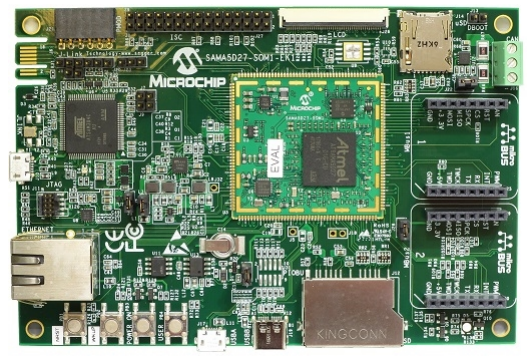
\includegraphics[scale=.7]{../pic/hw_top_view.png}
		\caption{Razvojna ploca SAMA5D27-SOM1-EK1 (pogled odozgo)}
		\label{fig:hw_top_view}
	\end{figure}


	SOM je potpuno opremljen industrijski sertifikovan kompjuter dizajniran za integraciju
	korisnicke aplikacije. SOM modul je namenski napravljen kao mala hardverska platforma
	opremljena sirokim spektrom modula za brzo povezivanje kako bi podrzali	projektovanje podrske
	za razne IoT (Internet of Things) aplikacija, prenosnih uredjaja, ali i aplikacija u
	industrijske svrhe. SOM integrise 1Gbit DDR2 SDRAM i QSPI memoriju kao 10/100 Mbit Ethernet
	interfejs. Takodje, SOM poseduje i 128 GPIO pinova (\#\# [lazarc]) koji	obezbedjuju pristup
	SOM-a za razlicite upotrebe. Svi GPIO pinovi su nezavisni, i mogu se konfigurisati kao ulazi
	ili izlazi, sa ili bez PULL-UP otpornika. Razvojna ploca poseduje i	sirok spektar periferija,
	kao i korisnicki interfejs i nacin za prosirenje funkcionalnosti, ukljucujuci i dva microBUS
	Click interjesa firme Mikroelektronika kojim se dobija mogucnost za	prosirenje funkcionalnosti
	svim modulima koje ova firma nudi u svom asortimanu.

	\begin{figure}[htb]
		\centering
		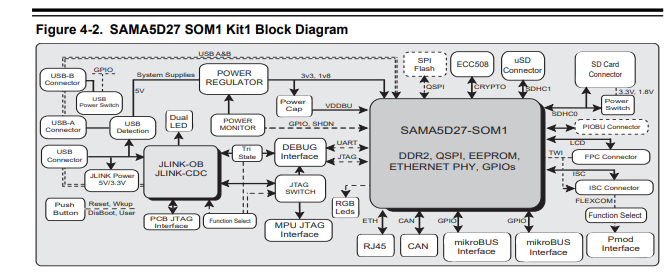
\includegraphics[scale=.7]{../pic/hw_modules.png}
		\caption{Moduli - Razvojna ploca SAMA5D27-SOM1-EK1}
		\label{fig:hw_modules}
	\end{figure}

	Na samom SAMA5D27-SOM1 postoje i:
	\begin{itemize}
		\item Ultra mali SIP (SAMA5D27-D1G-CU) koji sadrzi stedljivi SAMA5D27 Arm Cortex A5
		procesor i 1Gbit DDR2 SDRAM memoriju
		\item SST26VF064 64 Mb QSPI Flash memoriju
		\item 24AA02E48 2 Kb serijski E2PROM (Electrically Erased Programmed Read Only Memory) sa
		programiranom EUI identifikacijom pristupa
		\item MIC2800 cip za kontrolu napajanja
		\item KSZ8081RNA Ethernet Phy 10/100 MHz RMII
	\end{itemize}

	\begin{figure}[htb]
		\centering
		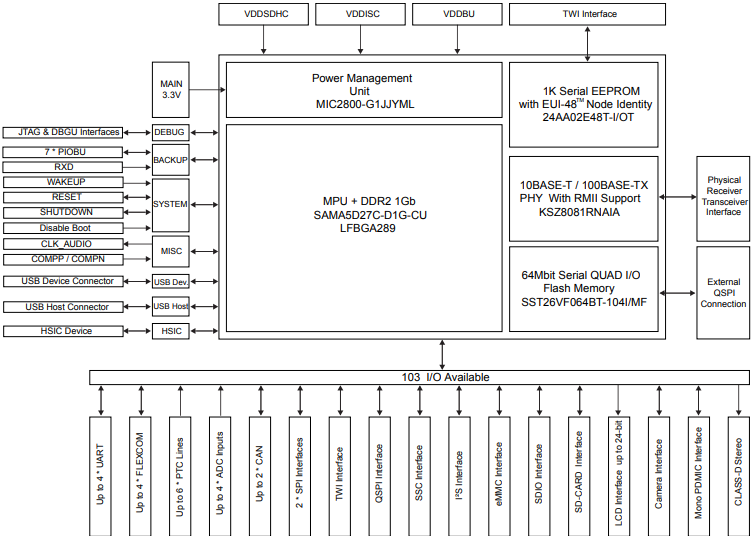
\includegraphics[scale=.7]{../pic/hw_som_modules.PNG}
		\caption{Moduli - SAMA5D27-SOM1}
		\label{fig:hw_som_modules}
	\end{figure}

	Razvojno okruzenje SAMA5D27-SOM1-EK1 je veoma mocno i moze se koristiti za sirok spektar
	aplikacija. Najcesce je izbor za razvoj aplikativnog softvera u namenskim racunarskim
	sistemima, uz koriscenje Embedded Linux operativnog sistema, i s tim ciljem se i bira. Za ovu
	implementaciju nije koriscen u tom smislu, vec je koriscen sa drugim operativnim sistemom kojim
	je moguce istaci neke druge njegove karakteristike. Ali ono sto je najvise interesantno za ovu
	primenu je postojanje TSU (Timestamping unit) za harversku podrsku PTP-a. I to u sklopu
	periferije za povezivanje preko Ethernet-a, cime je omugceno prepoznavanje PTP poruka koje
	dolaze na interfejs.

	\section{Time stamping unit - TSU}
	IEEE-1588 je standard za preciznu sinhronizaciju vremena u lokalnim mrezama. Radi se o razmeni
	preciznog vremena izmedju dva uredjaja u lokalnoj mrezi. PTP poruke se mogu prenositi preko
	IEEE802.3/Ethernet, IPv4 ili IPv6 protokola kako je to vec opisano u odeljcima pre. Periferija
	unutar razvojnog okruzenja GMAC oznacava tacku vremenske oznake poruke (na pocetku slanja i na
	kraju slanja) poruke. IEEE 802.1AS je podskup IEEE 1588 standarda. Jedina razlika je u adresi
	koja sluzi za slanje PTP poruka svim uredjajima u lokalnoj mrezi (Multicast). GMAC periferija
	je dizajnirana tako da prepoznaje poruke koje su kljucne za PTP protokol. Kao sto je vec
	navedeno, sinhronizacija izmedju dva uredjaja se izvodi u dva stadijuma, odredjivanje razlike
	(offset) izmedju dva sata (na strani Master i Slave uredjaja), nakon cega se salje tacno
	kasnjenje na linijama za prenos podataka, cime se tacno sinhronizuju dva sata. Hardverski
	moduli koji pomazu u ovoj razmeni poruka odredjuju tacno vreme kada je poruka stigla, i kada je
	poruka poslata. Sto je kljucno za odredjivanje vremena kojim se izracunavaju razlika i
	kasnjenje. Pojava ovih poruka uzrokuje prijavljivanje hardverskih prekida, tako da je moguce
	operisati sa vremenima koja se dobijaju tako da se dobija fina sinhronizacija vremena dva
	uredjaja.
	Podrska ovom protokolu u hardveru se ogleda u postojanju TSU(Timestamping unit) periferije koja
	se sastoji od tajmera i registara u koje se smestaju tacna vremena u trenucima kada stignu ili
	odu poruke koje su kljucne za dobijanje tacnog vremena. Prekid se prijavljuje kada se ovi
	registri osveze vremenom slanja ili primanja poruke bitne za PTP protokol.
	Tajmer je implemntiran kao 94-bitni brojac, u kome visih 48 bita broje sekunde, narednih 30
	bita nanosekunde, i preostalih 16 bita broje vreme ispod nanosekunda. Nizih 46 bita se prevrte
	(roll-over) kad se izbroji tacno jedna sekunda. Takodje, prijavljuje se hardverski prekid nakon
	sto se izbroji jedna sekunda. Vrednosti tajmera, kao i parametri za njegovo upravljanje, se
	mogu menjati softverski preko APB interfejsa. Tajmer se pokrece MCK taktom, koji je glavni takt
	unutar procesora, i njime se takodje moze manipulisati.
	Promene podesavanja tajmera unutar TSU su od velike vaznosti za tacnu sinhronizuju dva
	uredjaja. Ova periferija najvise utice na tacno vreme koje je potrebno sinhronizovati, i
	takodje daje informacije o tacnom vremenu na uredjaju koji se koristi. Vise detalja o samoj
	implemntaciji i koriscenju ove periferije bice dato u delu softverske implementacije.

	\newpage

	\chapter{Softverska implementacija}

	\newpage

	\chapter{Zaključak}

	\newpage

\end{document}
